\section{Metodologia}%
\label{sec:metodologia}

Para a condução deste trabalho, foi realizada uma pesquisa bibliográfica sobre o problema, incluindo a natureza das restrições e os limites superiores e inferiores possíveis para suas variáveis.

\subsection{Função Objetivo}

Com esse aprofundamento, compreendemos que o problema envolve a minimização da área da seção transversal das três barras que compõem uma treliça. Para evitar que o problema se torne multiobjetivo, a avaliação é feita considerando um peso fixo hipotético posicionado sobre a treliça, de forma que o único objetivo é minimizar o peso total da estrutura, mantendo sua capacidade de suportar tal peso.

Assim, seções transversais menores resultam em um peso menor e, consequentemente, em uma solução de melhor qualidade. Embora à primeira vista o problema pareça requerer três variáveis (uma para cada barra da treliça), a simetria estrutural exige que as barras diagonais tenham seções iguais, evitando tendências de giro que poderiam comprometer a integridade da estrutura. 

Dessa forma, as barras 1 e 3 devem ter a mesma área de seção transversal, reduzindo o problema para duas variáveis: \(x_1\) e \(x_2\), onde \(x_1\) representa as seções das barras diagonais e \(x_2\) a seção da barra horizontal.

\todo{Inserir figura ilustrativa do problema}

% \begin{figure}[!ht]%
%     \centering
%     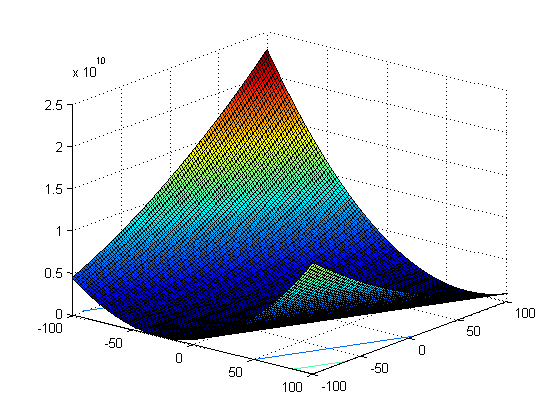
\includegraphics[scale=0.5]{img/f1.png}
%     \caption{Representação tridimensional da função \glsentryfull{f1} em duas dimensões. Fonte: \citeonline{cec2014}.}%
%     \label{fig:f1}
% \end{figure}

A função objetivo pode ser expressa como:

\begin{gather}
    \begin{align}
      \begin{split}
        y = \left( 2 \sqrt{2} \cdot x_1 + x_2 \right) \cdot 100
      \end{split}
    \end{align}
\end{gather}

\todo{colocar as unidades}

\subsection{Restrições}

O problema está sujeito a restrições de tensão, deflexão e flambagem
\todo{referencia}
, com um valor máximo permitido de 2 em todos os casos. Se \(g_x > 0\), ocorre uma violação da restrição, o que significa que a solução proposta não é viável estruturalmente.
As restrições são expressas pelas seguintes equações:

\begin{gather}
      \begin{subequations}
        \begin{align}
          \begin{split}
            g_1 = \frac{2 \left( \sqrt{2} \cdot x_1 + x_2 \right)}{\sqrt{2} \cdot x_1^2 + 2 \cdot x_1 \cdot x_2} - 2
          \end{split}
          \\
          \begin{split}
            g_2 = \frac{2 \cdot x_2}{\sqrt{2} \cdot x_1^2 + 2 \cdot x_1 \cdot x_2} - 2
          \end{split}
          \\
          \begin{split}
            g_3 = \frac{2}{x_1 + \sqrt{2} \cdot x_2} - 2
          \end{split}
        \end{align}
      \end{subequations}
\end{gather}

\subsection{Penalização}

Caso alguma das restrições \(g_1\), \(g_2\) ou \(g_3\) seja positiva, a restrição será violada, indicando que a solução é estruturalmente inviável. Para esses casos, são estabelecidos dois valores de penalização: \(\phi\) e \(\text{viol}\), que são adicionados à função objetivo. Esses valores positivos prejudicam a qualidade da solução, dado que se trata de uma função de minimização. 

O valor \(\phi\) é a soma dos valores que violam as restrições, enquanto \(\text{viol}\) representa o número de restrições violadas.

\begin{gather}
    \begin{align}
        \begin{split}
            \phi = \sum \max(g_i, 0)
        \end{split}
    \end{align}
\end{gather}

Onde \(g_i\) são as restrições \(g_1\), \(g_2\) e \(g_3\).

\todo{Adicionar subseção de segundo nível para a função objetivo penalizada}

A função objetivo penalizada é dada por:

\begin{gather}
    \begin{align}
        \begin{split}
            f(x) = y + w_1 \cdot \phi + w_2 \cdot \text{viol}
        \end{split}
    \end{align}
\end{gather}

Onde \(w_1\) e \(w_2\) são os pesos associados à cada forma de penalização e \(\text{viol}\) é o número de restrições violadas.

\subsection{Configuração dos Experimentos}

A seguir, apresentamos as constantes e parâmetros selecionados para a realização dos experimentos.

\subsubsection{Constantes}

As constantes utilizadas nos experimentos são listadas na \autoref{tab:constantes}.

\begin{table}[htb]
    \center%
    \begin{tabular}{l l}
        \bottomrule
        \textbf{Constante}    & \textbf{Valor} \\ \midrule
        Target               & Min            \\ \midrule
        Tamanho da população & 50             \\ \midrule
        Taxa de crossover    & 90\%           \\ \midrule
        Mutação              & Flip           \\ \midrule
        Taxa de mutação      & 5\%            \\ \midrule
        Elitismo (melhores)  & 10\%           \\ \midrule
        Elitismo (piores)    & 30\%           \\ \midrule
        Gerações             & 1500           \\ \toprule
    \end{tabular}
    \caption{Constantes utilizadas nos experimentos.}%
    \label{tab:constantes}
\end{table}

O algoritmo memético, por ser uma extensão do algoritmo genético, utiliza os mesmos parâmetros da \autoref{tab:constantes}, variando apenas o tipo de crossover e o número de gerações. Os parâmetros específicos do algoritmo memético estão listados na \autoref{tab:memetico}.

\begin{table}[htb]
    \center%
    \begin{tabular}{l l}
        \bottomrule
        \textbf{Constante}    & \textbf{Valor} \\ \midrule
        Taxa de exploração local & 0.5          \\ \midrule
        Máx. gerações locais   & 10            \\ \midrule
        Bits por parâmetro     & 4             \\ \midrule
        Tipo de crossover      & Um ponto      \\ \midrule
        Gerações               & 100           \\ \toprule
    \end{tabular}
    \caption{Parâmetros adicionais do algoritmo memético.}%
    \label{tab:memetico}
\end{table}

As variáveis de decisão, \(x_1\) e \(x_2\), que representam as áreas das seções transversais das barras, foram normalizadas para o intervalo de 0 a 1, garantindo consistência na avaliação dos resultados. A população inicial é gerada aleatoriamente dentro desse intervalo, e seu tamanho permanece fixo em 50 indivíduos ao longo de todas as gerações.

O operador de \gls{crossover} é aplicado com uma taxa de 90\%. A mutação, com uma taxa de 5\%, é realizada utilizando o método \texttt{flip}. O elitismo é aplicado a 10\% dos melhores indivíduos e a 30\% dos piores. No algoritmo genético, a execução ocorre por 1500 gerações, enquanto no algoritmo memético, por 100 gerações.

\subsection{Parâmetros e Variáveis}

Os experimentos foram conduzidos utilizando os parâmetros que apresentaram os melhores resultados nas etapas anteriores deste trabalho. Assim, a única parametrização dinâmica do experimento foram os pesos atribuídos a cada tipo de penalização.

Para garantir a robustez dos resultados, os experimentos foram repetidos 10 vezes para cada algoritmo.
